\documentclass[a4paper,12pt]{article}

% for manual date positioning
\usepackage{datetime}
\newdateformat{monthyeardate}{\monthname[\THEMONTH], \THEYEAR}

\usepackage{listings}

% from https://tex.stackexchange.com/questions/47175/scala-support-in-listings-package#47209
% "define" Scala
\lstdefinelanguage{Scala}{
  morekeywords={abstract,case,catch,class,def,%
    do,else,extends,false,final,finally,%
    for,if,implicit,import,match,mixin,%
    new,null,object,override,package,%
    private,protected,requires,return,sealed,%
    super,this,throw,trait,true,try,%
    type,val,var,while,with,yield},
  otherkeywords={=>,<-,<\%,<:,>:,\#,@},
  sensitive=true,
  morecomment=[l]{//},
  morecomment=[n]{/*}{*/},
  morestring=[b]",
  morestring=[b]',
  morestring=[b]"""
}

\usepackage{setspace}   % to change line spacing within a paragraph
%\usepackage{indentfirst}	% to indent first paragraph
\usepackage{graphbox}   % to give includegraph the align option
\usepackage[lmargin=2.00cm,tmargin=3.00cm,rmargin=3.00cm,bmargin=2.00cm,]{geometry}	% for margins
\usepackage[british,english]{babel}	% language
\usepackage{color}	% to specify colours

% for tikz macros
\usepackage{tikz}

% for trademark symbol
\usepackage{textcomp}

\definecolor{sepia}{RGB}{103, 24, 0}

% add float barriers to keep figures from being moved
% http://anorien.csc.warwick.ac.uk/mirrors/CTAN/macros/latex/contrib/placeins/placeins-doc.pdf
\usepackage{placeins}		

% for hyperlinks; colorlinks=true means change the text
% colour rather than adding a colourful border
\usepackage{hyperref} 	
\hypersetup{
  colorlinks=true,
  linkcolor=sepia,
  urlcolor=blue,
  citecolor=red
}

% this makes sure that captions only include the `:' character if your
% caption has extra text in it
\usepackage{caption}
\captionsetup[table]{name=Table}

% paragraph spacing
\setlength{\parskip}{\baselineskip}%

% for lists and margins
\usepackage{enumitem}

% for the author year referencing style, using biber as backend, in citations keep the 
% number of authors to one, then append 'et al.', in bibliography show all authors...
\usepackage[citestyle=ieee,style=authoryear,backend=biber,maxcitenames=1,maxbibnames=20,urldate=short]{biblatex}
\DeclareNameAlias{author}{last-first} % ... with all authors in the `surname, name' format
\addbibresource{bibliography.bib}
\renewcommand*{\nameyeardelim}{\addcomma\space}
\DeclareFieldFormat{urldate}{%
  (visited on: \thefield{urlday}\addspace%
  \mkbibmonth{\thefield{urlmonth}}\addspace%
  \thefield{urlyear}\isdot)}


%%%%%%%%%%%%%%%%%%%%%%%%%%%%%%%%%%%%%%%%%%%%%%%%%%%%%%%%%%%%%%%%%%%%%%

\begin{document}

\begin{titlepage}
  \center
  
  \vspace*{3cm}

  {
    \begin{spacing}{1.2}
      \LARGE The Design and Build of a Simple Personal Finance System, Focused
      on Budgeting and Expenditure Analysis
    \end{spacing}
  }

  \vfill
  
  Word Count: \emph{10,502}, excluding appendices.
  
  \vfill

  Claudius de Moura Brasil\\
  BSc Computing Project Report\\
  Birkbeck College, University of London

  May 2018

  This report is the result of my own work except where explicitly stated in
  the text. The report may be freely copied and distributed provided the source
  is explicitly acknowledged.
  
  \vfill

\end{titlepage}


\newpage
\pagenumbering{roman}
\section{Abstract} \label{sec:Abstract}
Personal finance systems exist in abundance nowadays, from open source to
proprietary ones. They all tend to revolve around a basic common theme:
providing accurate information about an individual's income and expenditure.
Beyond this, they tend to vary in which features are implemented. The system
designed and built for this project focuses on the use of the bookkeeping
principle of double entry and the concept of pattern matching to find effective
ways to cagetorise a user's expenditure, and provide them with relevant
financial information to assist in decision making.


\newpage
\tableofcontents

\newpage
\pagenumbering{arabic}
\section{Introduction} \label{sec:Introduction}

A system could be summarised roughly as a solution to one or more problems. One
of the first steps in order to build this kind of solution is to try to
understand the problem -- that is, try to map the requirements of the software.
Vaasen et al. (2009 \cite[cited][p.~8]{Boczko:2012:IAI:2331376}) suggests that
an accounting information system's main purpose is to provide information to
internal and external stakeholders. Although this refers to accounting systems
for businesses, it could be argued that this same definition can be employed to
define personal finance systems -- except that, in this case, the main
stakeholder would be the individual using the system (that is, the user). In
fact, one of the most widely known accounting systems available in the market,
Quicken\texttrademark, was conceived around the idea that there should be more
efficient and less tedious ways to organise one's personal financial
information than doing it manually (\cite{quicken2017about}). This project has
been developed based on similar ideas.

It seems fair to infer that nowadays most of a user's financial transactions
happen in ways that can be listed electronically (usually via their bank or
credit card statements) -- a study by Payments UK
(\citeyear{paymentsUK2017summary}), for example, indicates that there has been
a rise in debit card payments over the past few years, and that the volumes of
this type of transaction is likely to be higher than that of cash payments by
the year 2021. Therefore, an assumption has been made that the users will
require means of uploading a list of their financial transactions into the
system in an electronic format.

The system created for this project intends to do just this. Its main feature,
however, will be to allow the user to categorise expenditure based on patterns
in the entries' descriptions. Aside from this, there will also be a feature to
allow the user to view summaries of the income and expenditure over a period of
time, and another one to generate budget forecasts for future periods based on
the financial information already entered.

This report documents the work of the project. Each chapter delineates a
specific aspect of the development life cycle, which is in line with the
development process described in the following paragraphs. Chapter
\ref{sec:Requirements} outlines the identified requirements which were used as
motivation for the system to be developed; the contents of Chapter
\ref{sec:AnalysisAndDesign} shows further analysis and concomitant design of
the system and the solutions it brings; Chapter \ref{sec:Implementation}
outlines select aspects of the implementation stage which serve to emphasise
the techniques used to implement the designed logic, or highlights areas where
it was felt it was necessary to implement something slightly different that
what was designed.

The system developed for this project has been modelled after the principle of
\emph{double entry bookkeeping}, from the accounting domain, which states that
``money is never created or destroyed -- it merely moves from one account to
another'' (\cite[][Section 6.2]{fowler1997analysis}). More specifically, double
entry is the principle which ensures that every transaction always affects two
accounts, one being credited (Out) and one debited (In). An account, for the
scope of this project, refers either to a category created by the user, or to
the user's \emph{cash book} -- the contents of their bank account plus any
manual entry which they make. In bookkeeping, each account can be classified as
\emph{asset, liability, income} or \emph{expenditure}. Whether the account
increases or decreases will depend on which of these categories it falls under:
\emph{debits} will increase \emph{assets} and \emph{expense} accounts, and
\emph{credits} will increase \emph{liability, capital} or \emph{income}
accounts (\cite[][pp.~18-19]{wood2004book}).


Regarding the development method, an approach similar to that adopted by
Bennett et al.  (\citeyear[][p.~77]{bennett2010object}) regarding software
analysis an design has been employed, where no specific named methodology is
espoused, but concepts of object-oriented analysis and design were applied, in
an iterative and incremental fashion, using UML. More details about which
concepts were used and the methodologies which originated them can be found in
the following subsections.


The remaining definitions from \hyperref[appendix1]{Appendix I}, including
those of functional and non-functional requirements, will be employed when
trying to classify the requirements and model the problem domain. The initial
iterations will be focused more on the functional and usability requirements,
paying some attention as well to specific non-functional requirements such as
performance and security.

Throughout the report, the term \emph{domain} will be employed, as defined by
Evans (\citeyear[][p.~2]{evans2004domain}), to define the ``activity or
interest of its user'' -- the ``subject area to which the user applies the
program''. 

\hyperref[appendix3]{Appendix III} explains how to build and run the latest
version.


\newpage
\section{Requirements} \label{sec:Requirements}

\subsection{Business Case} \label{sec:Requirements.BusinessCase}
Any personal accounting system should be able to provide accurate and relevant
summaries of an individual's financial status. In order to do this, the user
needs to be able to supply the system with the necessary data, so that it can
be analysed and properly converted into knowledge.

The scope of the personal finance system developed for this project must
include a feature to allow a user to upload their bank and credit card
statements into it. Each transaction should be classified based on categories
which the user will create. The user should then be able to visualise a summary
of their income and expenditure by category and period, which should allow them
to have a concise and clear visibility of how much they have earned and spent
over any period of time. The category must be handled with care -- there should
not be a case where a user deletes a category and then all the entries in a
period are lost with it, but if a user wants to change the name of a category
they should be free to do so.

Since there may be other sources of income which the user may want to
categorise (such as breakdowns of cash transactions from pocket money), a
feature to allow for manual entries should also be made available. The user can
declare a lump sum, and then break it down among categories. The option should
allow them to choose whether the transaction is a credit or a debit from a
specific category, and then provide the corresponding debit or credit to a
category of their choice. For example, if the user withdraws \pounds50, and
spends half of it on weekly shopping and the other half on a cinema ticket,
they should be able to `credit' (withdraw) \pounds50 from the \emph{Bank}
category, and then `debit' \pounds25 to both \emph{Weekly Shopping} and
\emph{Entertainment} categories.

Once the system has enough data, it should be able to calculate a simple budget
and display it for the user. The budget can be a simple average of income and
expenditure over a long enough period of time, projected over the future
month/year -- it would only be used as a guideline for the user, anyway.

\subsection{Functional Requirements} \label{sec:Requirements.FunctionalRequirements}

Based on the description above, a few functional requirements were identified.
They are represented in the diagram on section
\ref{sec:Requirements.FunctionalRequirements.UseCaseDiagram} and the list,
wireframes and activity diagrams on section
\ref{sec:Requirements.FunctionalRequirements.UseCaseList}.

\subsubsection{Use Case Diagram} \label{sec:Requirements.FunctionalRequirements.UseCaseDiagram}
Use case diagrams are UML constructs which were developed by Jacobson et al.
(1992, cited \cite[][p.~154]{bennett2010object}). The use case diagram on
Figure \ref{fig:UseCaseDiagram} is used to illustrate the functional
requirements identified for this project:
\begin{figure}[ht!]
  \begin{center}
    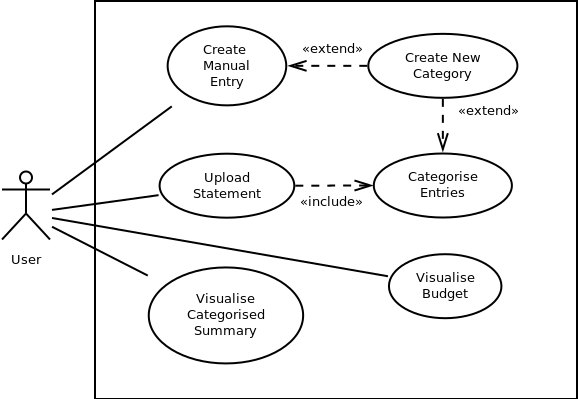
\includegraphics[width=14cm]{./contents/img/Use_Case_Diagram.png}
  \end{center}
  \caption{Use Case Diagram}
  \label{fig:UseCaseDiagram}
\end{figure}
\FloatBarrier



\subsubsection{Use Case List} \label{sec:Requirements.FunctionalRequirements.UseCaseList}
Table \ref{tab:UseCaseDescriptions} lists the descriptions for the use cases
listed above:
\begin{table}[ht!]
  \centering
  \begin{tabular}{|p{4cm}|p{12cm}|}
    \hline
    \textbf{Use Case}&\textbf{Description}\\
    \hline
    Upload Statement&The user must be able to upload a list of their
                     financial transactions, most likely their bank
                     or credit card statements, in a valid format, and all
                     entries should be categorised based on specific patterns\\
                    &\emph{Includes}: Categorise Entries\\
    \hline
    Create Manual Entry&The user should be able to create a manual transaction for
                        income or expenditure, include a date, amount and
                        description, and classify it among existing categories
                        or create new ones in the
                        process\\
                        &\emph{Extends}: Create Category\\
    \hline
    Visualise Categorised Summary&The user must be able to visualise
                                  a summary of their income and expenditure
                                  over a period of time\\
    \hline
    Calculate Budget&The user must be able to visualise a budget for future
                     periods based on their income and expenditure data 
                     already entered\\
    \hline
    Categorise Items&Analyse the current entry and assign it to a category\\
                    &\emph{Extends}: Create Category\\
    \hline
    Create Category&Creates a new category with the name suggested by the
                        user\\

    \hline
  \end{tabular}
  \caption{Use Case Descriptions} \label{tab:UseCaseDescriptions}
\end{table}
\FloatBarrier

The \emph{Estimate Tax} feature  was not included in these requirements, as the
time constraints would not allowed for it to be implemented, but its
specifications can be seen in \hyperref[appendix4]{Appendix IV}.

\subsubsection{Designing the User Experience with Wireframes}
The wireframe below (Figure \ref{fig:Wireframe.CreateManualEntry}) was created
to better illustrate the \emph{Manual Entry} requirement from the point of view
of the user. It shows an example of an entry for a laptop and a licence for a
proprietary operating system, which can then be broken down among different
categories. The user has the option to use the percentage or the amount boxes
in order to provide a breakdown, and they can also add new lines if more than
one is required -- the example shows two lines, but the default would be one.
Under the category search box, if the user types a category name that does not
exist they will be asked if they want to create a new one:
\begin{figure}[ht!]
  \begin{center}
    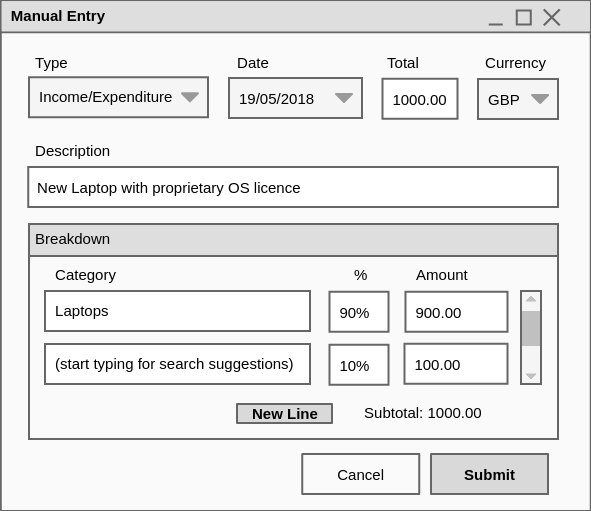
\includegraphics[width=14cm]{./contents/img/Wireframe_-_Manual_Entry.png}
  \end{center}
  \caption{User interface wireframe for \emph{Create Manual Entry} use case}
  \label{fig:Wireframe.CreateManualEntry}
\end{figure}
\FloatBarrier

And in order to better understand the relationship between \emph{Upload
Statement} and \emph{Categorise Entries}, the activity diagram below (Figure
\ref{fig:AD.CategoriseEntries}) was developed:
\begin{figure}[ht!]
  \begin{center}
    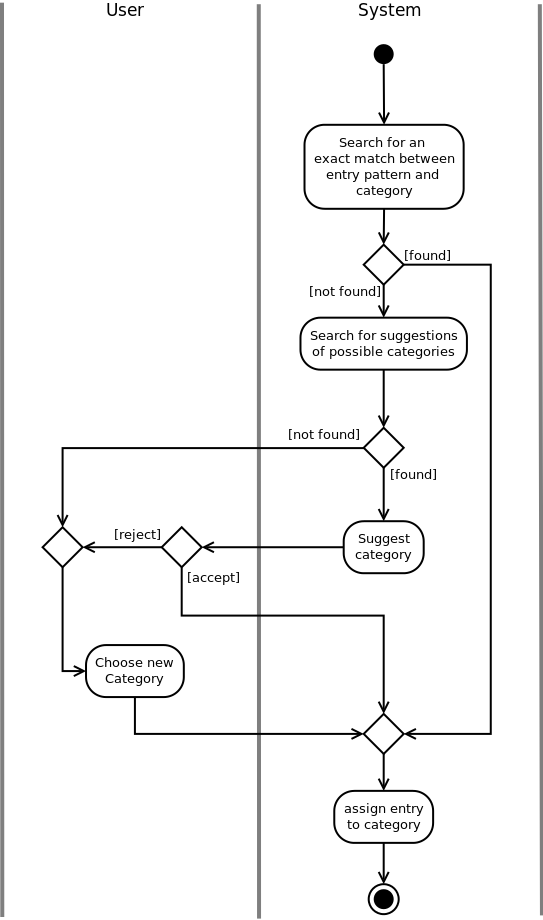
\includegraphics[width=11cm]{./contents/img/Activity_Diagram_-_Categorise_Entries.png}
  \end{center}
  \caption{}
  \label{fig:AD.CategoriseEntries}
\end{figure}
\FloatBarrier

At the first few iterations, in order to provide a minimum viable product, the
process of categorisation will be a blocking one consisting of multiple calls
being made to the process above -- for each call, the process will block awaiting
user input when a category is not found. However, there are plans for future
iterations where this process could be optimised by concurrency, and if there
is enough time a more appropriate interface will be built for such a case.

The initial interface for uploading a statement should be a simple one, such as
the one below
(\ref{fig:Wireframe.UploadStatement}), and at least initially the interface for
manual entry will be used whenever user input is required:
\begin{figure}[ht!]
  \begin{center}
    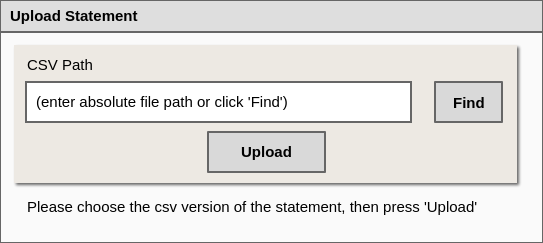
\includegraphics[width=12cm]{./contents/img/Wireframe_-_Upload_Statement.png}
  \end{center}
  \caption{}
  \label{fig:Wireframe.UploadStatement}
\end{figure}
\FloatBarrier

Below (Figure \ref{fig:Wireframe.VisualiseCategorisedSummary}) is also a
wireframe illustrating the GUI for \emph{Visualise Categorised Summary}. The
user should have an option to select the dates and, if they only want to see
one category, the category itself:
\begin{figure}[ht!]
  \begin{center}
    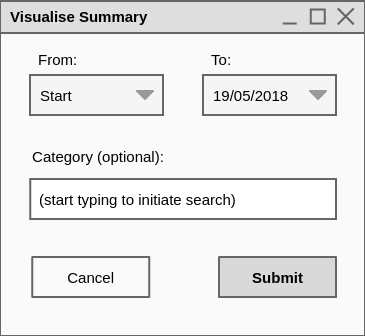
\includegraphics[width=8cm]{./contents/img/Wireframe_-_Visualise_Summary.png}
  \end{center}
  \caption{}
  \label{fig:Wireframe.VisualiseCategorisedSummary}
\end{figure}
\FloatBarrier

The dates field should allow them both to type a date or choose it from a drop
down calendar. If no values are entered, the system will return a summary of
all categories on the system.




\subsection{Non-Functional Requirements} \label{sec:Requirements.NonFunctionalRequirements}
At this iteration, no significant non-functional requirements were identified,
so they were not included in this report.


\newpage
\section{Design} \label{sec:Design}



\newpage
\section{Implementation} \label{sec:Implementation}

The initial Minimum Viable Product (MVP) was implemented with major differences
from the design outlined in chapter \ref{sec:AnalysisAndDesign}.  The most
visible one is the fact that (what is mainly) the \emph{Mediator} pattern
(\cite[][Ch.~9,~Location~3594]{nikolov2016scala}) has been used in order to
implement the dialogue between the presentation and other layers using a
feature which resembles the MVC architecture, as mentioned in chapter
\ref{sec:AnalysisAndDesign}. Normally, this type of architecture is implemented
in order to make sure that multiple views can refer to the same core
functionality (or model) without actually implementing that functionality
themselves, which allows the view to be responsible for presentation and the
model for liaising with the business logic through a controller. This also
allows the controller to update multiple existing views based on what input was
received from one view (\cite[][p.~381]{bennett2010object}). The difference in
the implementation for this project is that this last feature, essentially, was
not implemented, since only one view exists at one time.

It is noticeable that the interface for manual entry available is different
than that shown in Figure \ref{fig:Wireframe.CreateManualEntry} is not exactly
the one implemented: the feature to add a new line to the breakdown is missing,
which makes the percentage of income irrelevant. This was once again due to
time constraints, and will have to perhaps be done at a further iteration.
Another difference is the fact that there was not enough time to implement a
mechanism to suggest categories to the end user, so this will have to be left
for a future iteration, outside of the scope of this report.

In the implementation phase of this project, the components were segregated
into packages (each of which represents one of the layers mentioned in Chapter
\ref{sec:AnalysisAndDesign}) and sub-packages. Each sub-package has been
implemented so that it does not have any knowledge of the super-package, but
rather exposes and depends on interfaces which exist within itself. The
super-packages, then, implement the interfaces of the sub-packages, which
allows them to interact with the sub-package components. The \emph{Mediator}
pattern was implemented at the default package level by the
\emph{InteractionMediator} and \emph{PersistenceMediator} objects, both of
which also happen to represent Scala's native implementation of the
\emph{Singleton} pattern (\cite[][Ch.~6,~Location.~2242]{nikolov2016scala}).
The following subsections will give more detail into the inner workings of the
application and the techniques used to build it.

\subsection{Presentation Layer} \label{sec:Implementation.Presentation}
In the presentation layer, for this MVP, the \emph{Scala Swing} package was
used to design the \emph{view}. The package itself consists of Scala wrappers
for the \emph{Java Swing} package, and one of the reasons why it was chosen was
that, as with many other GUI packages, it already comes with an implementation
of the \emph{Observer Design Pattern} (\cite[][p.~293]{gamma1995design}) in its
capacity to react to events (\cite[][p.~5]{maier2009scala};
\cite[][Ch.~9,~Location~3731]{nikolov2016scala}).

The entry point of the application is the \texttt{App} object, in the main
package. This application works as a main method, and its only task is to
call the \texttt{InteractionMediator.startup} method, which will send a
message through the \texttt{PresentationMediator} instance returned by the
\texttt{PresentationBuilder} to start the view.

\begin{sloppypar}
  In its current implementation, the view is started by the \texttt{MainWindow}
  class, which extends the \texttt{scala.swing.MainFrame} class. A
  \texttt{MainFrame} is a Swing \texttt{Frame} -- ``a window containing
  arbitrary data'' (\cite[][Ch.~34,~Section~34.1]{odersky2016scala}) -- that
  can send a signal to terminate the application when closed.
  \texttt{MainWindow} also has implementations of other methods to allow the
  application to close gracefully, all of which were inspired by the
  \texttt{SimpleSwingApplication} of the scala package
  (\cite[][p.~2~\&~3]{maier2009scala}). The author chose not to make the first
  extend the latter was because it would have inherited the main method of the
  super-class, which, considering that it would be another entry point to the
  application, could cause confusion when trying to run the application (not to
  mention the fact that this is not the responsibility of the
  \texttt{MainWindow} class).
\end{sloppypar}


As mentioned in the beginning of this chapter, each sub-package has been
designed so that it does not have to depend on the packages which envelop it.
The diagram below (Figure \ref{fig:PresentationMVC}) illustrates this using the
interaction between the \texttt{InteractionMediator}, \texttt{SwingAmbassador}
and the \texttt{presentation.swing} package and sub-packages as an example:

\begin{figure}[ht!]
  \begin{center}
    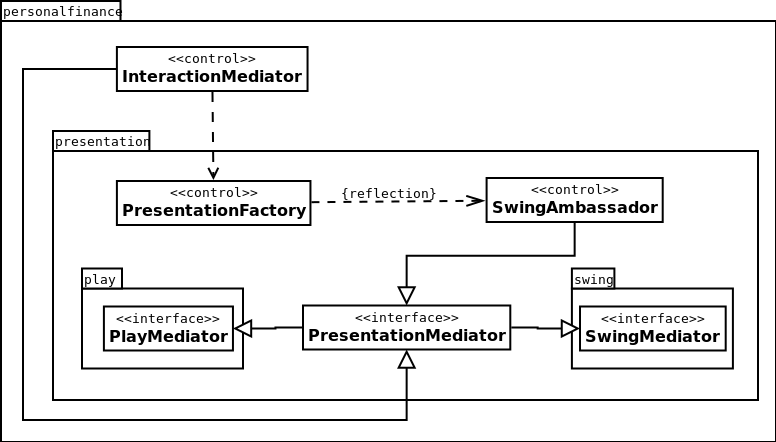
\includegraphics[width=15cm]{contents/img/Package_Diagram_-_Presentation_MVC.png}
  \end{center}
  \caption{}
  \label{fig:PresentationMVC}
\end{figure}
\FloatBarrier


\begin{sloppypar}
  In order to preserve encapsulation, specifically for the \texttt{swing}
  package, only the \texttt{MainWindow} controller and \texttt{SwingMediator}
  interface are exposed to the outside world, with the first having a
  constructor dependency on the latter. This means that, in order to interact
  with the components of the package, any external classes will need to
  implement the \texttt{SwingMediator} interface. This is also useful if the
  \texttt{presentation.swing} package is to be extracted and used as a library
  in another project, and also leaves room for the \emph{Adaptor} pattern
  (\cite[][p.~139]{gamma1995design}), if it needs to interact with other
  objects which do not necessarily implement the interface upon which it
  depends.
\end{sloppypar}

One feature also noticeable in Figure \ref{fig:PresentationMVC} is the fact the
\texttt{personalfinance} package is unaware of which of the view's
implementation it is interacting with. The modified version of 
\emph{Builder} pattern (\cite[][pp.~37-38]{lokke2009scala}) implemented on
\texttt{PresentationBuilder}, which uses reflection to determine what
implementation to build, allows for the view itself to be decided with the use
of an external \texttt{.properties} file. This allows for the actual
implementation which will be delivered by the Factory to change without the
code having to be recompiled, which introduces flexibility to the application.
The \texttt{play} package is only a placeholder at this point, as due to time
constraints it was not possible to actually implement it, but it is there to
exemplify how the project can be further extended.

Another element not seen in the diagram but which is present in the code is the
fact that the dependency of the \texttt{MainWindow} class on the
\texttt{SwingMediator} interface exists in the constructor, as seen in the code
listing below:
{
  \small
  \lstinputlisting[
    language=Scala,
    firstline=7,
    lastline=7,
    caption={ }
  ]{../code/src/main/scala/personalfinance/presentation/swing/MainWindow.scala}
}

This is an attempt at implementing the principle of \emph{Dependency Injection}
through \emph{Constructor Injection} (\cite[][]{fowler2004inversion}). In the
case of this project, the advantage of this simple piece of code is tremendous,
especially because the fact that the \texttt{MainWindow} class does not have to
instantiate a mediator -- it simply relies on the fields published by the
\texttt{SwingMediator} trait. Likewise, the fact that the
\texttt{InteractionMediator} singleton object has a dependency on the
\texttt{PresentationBuilder} only, allows for the actual implementation of the
view to change without it having to change.


The approach described above has an inherent risk due to Scala's \emph{mixin}
composition. Essentially, since trait \texttt{PresentationMediator} inherits
from multiple traits, any future extension to implement a new view would have
to keep in mind that \texttt{PresentationMediator} will be implementing the
behaviour of the last trait it implements in the source code. So any
refactoring of this trait which extends other traits may generate unexpected
behaviour, if this is not taken into consideration.


\subsection{Business Logic} \label{sec:Implementation.BusinessLogic}

The business logic layer is the one which adhered more firmly to the model
designed in section
\ref{sec:AnalysisAndDesign.BusinessLogic.FinalClassDiagram}. The following are
a few highlights from the implementation which are worth mentioning.

\subsubsection{Scala Case Classes and the Prototype Design Pattern} \label{sec:Implementation.ScalaCaseClasses}
One of the benefits of Scala are its case classes. Not just are they very
useful for pattern matching, but also come with a few perks such as the
\texttt{copy} method. This method allows for an object to be copied with some
or all its members modified. It could be said that it is a language-native
implementation of the \emph{Prototype Design Pattern}
(\cite[][Ch.~6,~Location~2461]{nikolov2016scala}), and throughout the
implementation and testing stage it proved to be a useful asset.

One of its many utilisations can be seen in the \texttt{Transaction} class, as
one of the tools used to add entries to a \texttt{Category} without having to
change the state of a specific instance -- more similar to what is done in the
\emph{Functional Programming} paradigm:
{
  \small
  \lstinputlisting[
    language=Scala,
    firstline=35,
    lastline=40,
    caption={
      extract of the \texttt{Transaction} class showing the \texttt{copy()}
      method in action
    }
  ]{../code/src/main/scala/personalfinance/businesslogic/transaction/Transaction.scala}
}


In order to be concise where possible, where it was felt that the domain's
requirements were captured accurately and was estimated that they are not
likely to change, high level modules are depending directly on classes rather
than interfaces. This can be seen as being in direct violation of the
\emph{Dependency Inversion} principle of SOLID
(\cite[][]{martin1996dependency}), which some would consider to be a ``risky'''
move (after all, it is not always possible to predict which requirements will
and which will not change), but others would believe that this was acceptable
for more static requirements. The author decided to follow the latter.

\begin{sloppypar}
  However, this principle was still employed where it seemed beneficial to
  follow it -- for example, in areas where it was felt that the implementation
  of certain algorithms could be further optimised in future iterations. This
  is the case with \texttt{transaction.RegexDateStringParser}: this class
  implements the \texttt{transaction.dates.DateStringParser} trait, upon which
  the higher level modules which use dates will depend. This is an example of
  one of the places in the code where the \emph{Dependency Inversion} principle
  can be seen, but it is not the only one.
\end{sloppypar}


\subsubsection{The engine behind it all: the \texttt{Classifier}}

Another example of \emph{Dependency Inversion} (though not of \emph{Dependency
Injection}) is the \texttt{Classifier} trait, and the class implementing it:
\texttt{StringClassifier}. The \texttt{InteractionMediator} declares a variable
of the first type, and then instantiates it with the latter. Therefore,
although it still depends on the abstraction, it also has a dependency on the
implementation, which would mean that in order to change it a slight
refactoring would be necessary.

For this implementation, \texttt{StringClassifier} was built using longest matching
prefix to match entries to categories: patterns are matched to the start of the
description of every entry, starting from longest pattern to the shortest. This
is so that if there is, for example, a pattern ``Laptop for parent'' which
would match to category ``Gifts'', and another pattern ``laptop'', for category
``personal equipment'', then entries with the description ``Laptop for
Girlfriend'' would not be picked up by the shorter match for laptop. Below is a
code listing which shows how this was implemented:
{
  \small
  \lstinputlisting[
    language=Scala,
    firstline=30,
    lastline=64,
    caption={
      Extract of the \texttt{StringClassifier} class, showing the algorithm currently
      used to match Entry descriptions' prefixes against patterns
    }
  ]{../code/src/main/scala/personalfinance/businesslogic/Classifier.scala}
}

As mentioned on the code listing above, the \emph{longest matching prefix} is
achieved by sorting all the patterns by length, from longest to shortest, then
trying to match them against the prefix of the entry description in the same
order. This way, even if an entry would be a match against more than one
category, the pattern with the longest matching prefix will still be the first
match.

One other interesting feature which can be seen in the above listing is how
much is being done using the native \texttt{flatMap} and \texttt{foldLeft}
methods of Scala collections. The \texttt{map} function and its derivates are
normally implemented by types which can be classified as \emph{Functors} in
scala. Functors are challenging to explain concisely, but for this report it
should suffice to say that they are \emph{classes which implement the}
\texttt{map} \emph{method and conform to a set of laws called} \textbf{functor
laws}. The \texttt{foldLeft} method of the collections are also an indication
that they can be classified as \emph{monoids}, which are another construct
brought over from mathematics. The main point of mentioning these is because
they are one of the things which makes the functional paradigm so powerful:
these constructs create a common interface which allows for the different types
with which they are associated to be interacted with in a common way -- that
is, a lot can be achieved with only a few lines of code
(\cite[][Ch.~1,~Location~4243~\&~703]{nikolov2016scala}). Not just this, but
the immutability of the instances within them also makes it easy to perform
these operations in parallel and, although this parallelism has not been
explicitly implemented in this iteration, the author felt it was worth
mentioning them in this section.

\subsection{The Presentation Layer}

The presentation layer is another one where decoupling and reflection can be
observed. The package is accessible via the \texttt{PersistenceBridge} class,
which uses reflection to instantiate one of the classes which implements the
\texttt{ConnectionType} trait. This is an implementation of the \emph{Strategy}
pattern (\cite[][p.~80]{lokke2009scala}), which allows for the database vendor
to be changed without the code having to be recompiled. At the moment, the only
dialect implemented is \emph{MySQL}, but a placeholder can already be seen for
the \emph{H2} database.

It is also worth noticing that the operations currently being executed by the
implementation have a lot of room for improvement: many of the queries and
updates which could be grouped together and sent to the database in batch are
still being done individually. This does not have a huge impact on performance
with a local database, but might cause issues with remote ones. Further
iterations of the application should focus on optimising this.

Another pattern which can be observed in this layer is the \emph{Value Object}
pattern, which will be discussed in more detail below.

\subsubsection{Algebraic Data Types and the Value Object Pattern} \label{sec:Implementation.ADTAndValueObject}
Throughout the code, examples of Algebraic Data Types can be seen. These appear
in the form of sealed traits and case objects, and are normally used when
instances need to be passed around as values, but also contain information which will
be relevant to the code. Examples of these can be found in the
\texttt{ConnectionType} hierarchy, where the number of possible instances for
each case class would classify the trait and its subtypes as \emph{Product
Types} (\cite[][p.~411]{wampler2015programming}). The code listing below
illustrates this:

{
  \small
  \lstinputlisting[
    language=Scala,
    firstline=9,
    lastline=9,
    caption={
      extract of the \texttt{ConnectionType} hierarchy showing the case classes
      used as value objects
    }
  ]{../code/src/main/scala/personalfinance/persistence/connections/ConnectionType.scala}
}
...

{
  \small
  \lstinputlisting[
    language=Scala,
    firstline=39,
    lastline=40
  ]{../code/src/main/scala/personalfinance/persistence/connections/ConnectionType.scala}
}
...

{
  \small
  \lstinputlisting[
    language=Scala,
    firstline=90,
    lastline=91
  ]{../code/src/main/scala/personalfinance/persistence/connections/ConnectionType.scala}
}
...

Algebraic data types could be said to be the natural implementation of the
Value Object design pattern. This pattern is used widely for comparison of
objects not by their identities, but rather by their values. They consist of
small, immutable objects, and the instances of the case classes can be
classified as just those (\cite[][Ch.~8,~Location~3068]{nikolov2016scala}).


\subsection{Application Output}

With the current version of the project, the main visible benefit which can be
seen is how it summarises income and expenditure by category, and uses this
information to display breakdowns by category and simple budgets to the end
user. The following is an example of how this can be achieved.

For this example, the user in question wants to upload the following bank
statement:
\begin{figure}[ht!]
  \begin{center}
    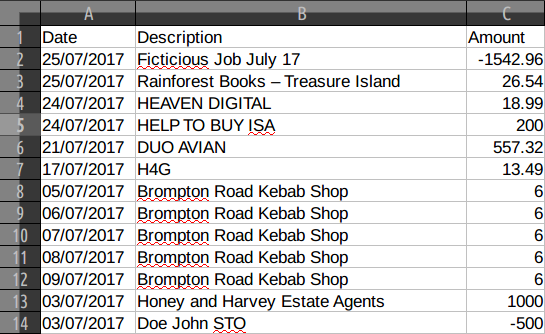
\includegraphics[width=10cm]{./contents/img/jul17_statement.png}
  \end{center}
  \caption{}
\end{figure}
\FloatBarrier

As can be seen from the above, there are multiple lines with the same
description. This is where the classifier will be most useful.

The user starts the application, and is greeted with the below interface:
\begin{figure}[ht!]
  \begin{center}
    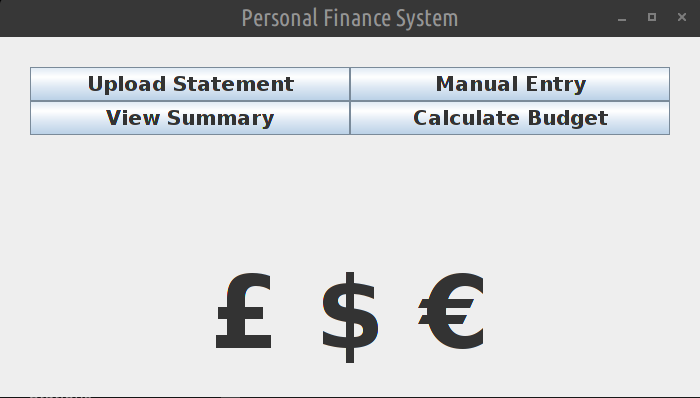
\includegraphics[width=14cm]{./contents/img/home_screen.png}
  \end{center}
  \caption{}
\end{figure}
\FloatBarrier

They choose the `Upload Statement' option, and point to the file containing the
statement:
\begin{figure}[ht!]
  \begin{center}
    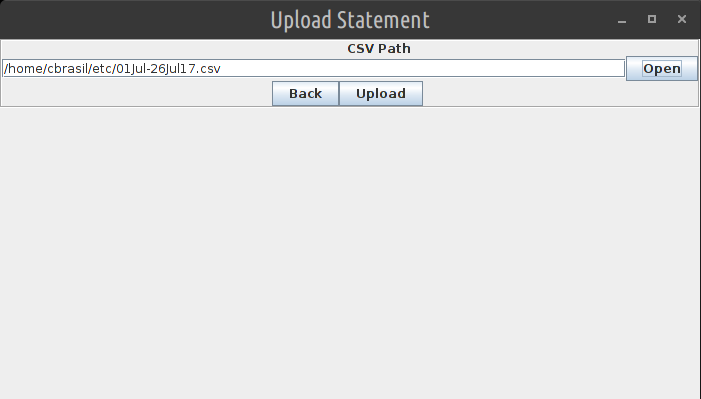
\includegraphics[width=14cm]{./contents/img/upload_statement.png}
  \end{center}
  \caption{}
\end{figure}
\FloatBarrier

When they click `Ok', this should trigger the sequence of events which will
attempt to classify the transactions. Each time the system encounters a
description it cannot match to an existing category, it will prompt the user
for input using the \texttt{CreateCategory} view. Below is an extract of when
trying to classify the income from the user's fictitious job:

\begin{figure}[ht!]
  \begin{center}
    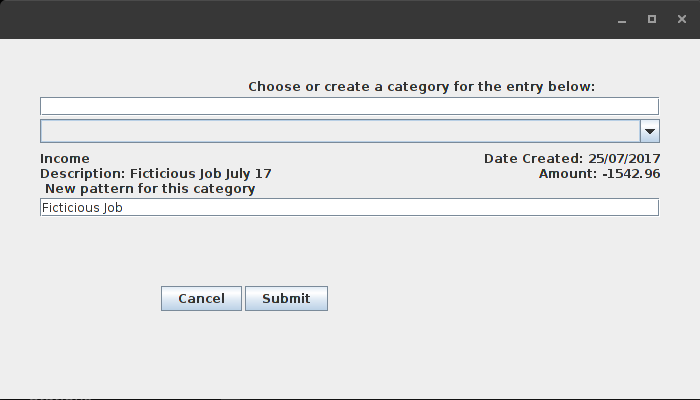
\includegraphics[width=14cm]{./contents/img/fictitious_job.png}
  \end{center}
  \caption{}
\end{figure}
\FloatBarrier

As can be seen from the above, by simply removing the date form the
description, the user will ensure that any future income is immediately put in
the same category as they choose for this one.

After all the categories have been entered, the user should be able to view a
summary by categories for that month, which will look something like the below:

\begin{figure}[ht!]
  \begin{center}
    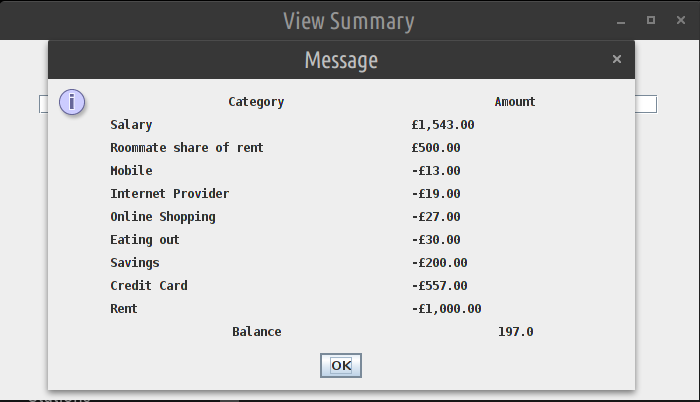
\includegraphics[width=14cm]{./contents/img/view_summary.png}
  \end{center}
  \caption{}
\end{figure}
\FloatBarrier


As it can be seen, the balance for that month is positive, showing the user
spent less than they earned for that month. 

After a whole year's worth of statements have been entered, the user should be
able to request a monthly budget. An example of what they would see can be seen
below:

\begin{figure}[ht!]
  \begin{center}
    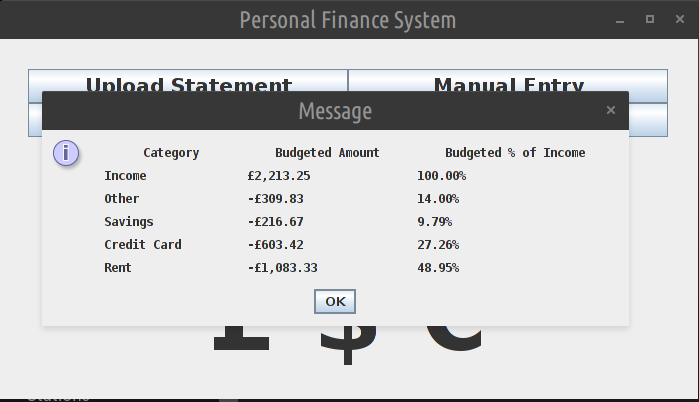
\includegraphics[width=14cm]{./contents/img/calculate_monthly_budget.png}
  \end{center}
  \caption{}
\end{figure}
\FloatBarrier


\newpage
\section{Testing} \label{sec:Testing}

As can be seen in the test suites implemented, the testing for this project was
an attempt at Behaviour-Driven Development (BDD), which is a form of
Test-Driven Development that focuses on trying to write tests by including
descriptions of the expected behaviour, which is also an attempt to make the
code more readable (\cite[][Ch.~1]{wynne2017cucumber}). The main library used
for testing was \texttt{ScalaTest}, ``an extensive BDD suite with numerous
built-in specs'' (\cite[][p.~21]{hinojosa2013testing}). Some of Scala's native
features also make it easy to write more readable tests, such as its infix
notation, which work well with the members of the \texttt{FlatSpec} class and
\texttt{Matchers} trait.

Most of the automated testing consist of integration tests, since more groups
of objects are being tested together but not necessarily the whole application.
This was chosen where it felt it would be beneficial to test how well the more
heavily integrated objects interacted. Whenever it was appropriate, mocks of
other objects were used, as can be seen in the \texttt{StringClassifierTester}
class. The \emph{Mockito} libraries were used for object mocking, as they work
well with \texttt{ScalaTest}, with the aid of Scala's \texttt{MockitoSugar}
trait, to aid with the syntax (\cite[][pp.~102-106]{hinojosa2013testing}).

The automated tests cover mostly the persistence and business logic layers, but
unfortunately not much was done with the presentation layer due to time
constraints. For the persistence layer, a test database schema was created, and
it needs to be loaded into a \emph{MySQL} database before it can be used. The
specifications for these need to be entered into \texttt{.properties} files
before running the tests, otherwise they will fail. Each time they run, any
changes made to the test database will be overwritten by the persistence
helper, which ensures consistency. The only reason this was done with
\emph{MySQL} for the current implementation is that the database is local,
therefore performance is not significantly affected. However, for future
iterations a portable database would be more suitable for persistence layer
testing.

Since TDD was used, in the vast majority of cases the tests were implemented
before the classes being tested were written. The classes were then written and
refactored until the tests were satisfied. In some cases, further tests were
written where it was noticed that more specific behaviours were required of
particular classes. After the tests were written, they behaved like a harness
which allowed for any further necessary changes to be made with confidence, and
helped to speed up the implementation phase
(\cite[][pp.~x-xi]{hinojosa2013testing}). The result of running the tests at
the time of writing can be seen in \hyperref[appendix4]{Appendix IV}.


Whenever `on-the-fly', manual tests were needed, these were done using the
Simple Build Tool (SBT) console feature. This feature is a very interesting
combination of Scala's Read-Eval-Print-Loop (REPL) with the build tool's
ability to quickly integrate all necessary dependencies into a REPL console
session (\cite[][p.~1]{hinojosa2013testing}). The advantage of testing in this
manner was that it was possible to run a session with compiled code incomplete
classes and test different aspects of their behaviour which did not seem fit
for automated testing.


\clearpage
\section{Reflections} \label{sec:Reflections}

\subsection{Expert Systems} \label{sec:Reflections.ExpertSystems}
Originally, the author did not know about expert systems when the idea for this
project was conceived. However this concept was found during the literature
search and review, and many of the patterns of what an expert system does and
what this system is supposed to do were identified to be similar. This led to
the conclusion that the project has the potential to become an expert system,
even if just with a budgeting tool. The expert knowledge being provided by it
for its first iteration includes:
\begin{itemize}
  \item
    Double entry bookkeeping;

  \item
    Budgeting by category.
\end{itemize}

It achieves the above by separating the inference engine, which is the tool
responsible for knowing how to apply double entry to transactions, from its
knowledge base which is the information input by the user -- for example, if
the user tells the system a manual entry is income, the system will know to
debit the cash book, and credit the category in question.

Brown et al. (\citeyear{brown1990expert}) declare that the heuristics used by a
financial planning system can be interpreted as a ``rule of thumb'' to be
applied to a problem which will normally result in a correct solution for it.
In the same article it is also stated that ``an expert system is most commonly
and most effectively used as an advisor to a human decision maker''. I this is
considered as the measure by which classify an expert system, then the
budgeting tool alone might qualify this system as one.

\subsection{Use Case Templates} \label{sec:Reflections.UseCaseTemplates}
Originally, no template was used to document the use cases. The intention was
to provide better ones at a later iteration, perhaps by researching the ones
mentioned by Bennett et al. (\citeyear[][p.~157]{bennett2010object}), but
unfortunately there was not enough time, so the little there was had to be
dedicated to the software itself.

\subsection{Iterations within the analysis and design iteration}
The analysis and design stages of the first iteration was delayed due to
multiple `trials and errors' within it. Appendices \ref{appendix2} and
\ref{appendix3} show a examples of different models which had been incorporated
into the final design, but which were later changed even before the
implementation started -- that is, even before any coding was done. This caused
a reflection on whether the development method was truly iterative, and whether
or not it was more similar to the Waterfall model.

\subsection{Dependency Injection} \label{sec:Reflections.DependencyInjection}
Very often during the implementation it was felt that better dependency
injection could be achieved. In classes such as those found in the
\texttt{TransactionsValidators.scala} file there was constant hard-coded
dependency to the \texttt{validation} package. In this instance, a framework
such as \emph{Spring} or \emph{Guice} would have been useful, but unfortunately
time constraints made it unlikely for the author to implement these into the
project. As a result, there is more tight coupling than there could be, but
wherever possible an effort has been made to pass the dependencies as
constructor or method parameters, so as to facilitate testing, among other
things.

\subsection{Validation} \label{sec:Reflections.Validation} 
\textbf{TODO: see if this is still the case at the end of the project}
A lot of thought has been put into where validation should happen. For example,
the constraints of \texttt{Transaction}, \texttt{Category} and \texttt{Entry}
which were used to enforce \emph{double-entry} could have been implemented at
database or application levels, or both. Initially they were implemented in the
business logic.



\clearpage
\printbibliography[heading=bibintoc]

\newpage
\section{Appendix I: Types of Requirements and the use of UML} \label{appendix1}

Bennett et al.
(\citeyear[][pp.~140-142]{bennett2010object}) categorises requirements as being
of three types:

\begin{description} \item[Functional Requirements]
    The system's functionality -- what it is expected to do.
    
  \item[Non-functional Requirements]
    How well the system delivers its functionality. These requirements are
    related to the performance, scalability, availability, recovery time,
    security, and others.

  \item[Usability Requirements]
    These relate to how effectively, efficiently and satisfactorily users can
    achieve their goals in the existing system. User interfaces can play a big
    part in meeting these requirements.
\end{description}

\subsection{The use of Universal Modelling Language (UML) constructs}
\label{sec:Introduction.methodology.uml}

UML is a modelling language created with the intention of providing system
architects, software engineers and developers with a common set of modelling
tools, with a defined syntax, which would help them better analyse and design
software-based systems, and to model business and similar processes
(\cite[][p.~43]{omg2015uml}). It defines several constructs which have been
employed throughout this report in order to model the specifications of the
system, such as Use Case, Activity, Class, Sequence and Communication Diagrams.  

In the class diagrams used, some thought was given to how to model the
relationships between entities. In the end, it was decided that transitory
relationships should be modelled as dependencies, and more permanent ones would
be modelled as associations.


\newpage
\section{Appendix II: Previous versions of analysis patterns} \label{appendix2}
Below is a previous version of analysis patterns. It was decided that keeping
track of \emph{balance} was not something worth pursuing, since the main point
of the application is for users to choose a period of time and then look at a
summary of expenditure in there.

The first analysis patterns which seem appropriate are the \emph{Account}
pattern, used to create the \emph{Category} entity class, and the
\emph{Quantity} pattern for the \emph{Amount} entity class
(\cite[][Sections~6.1~\&~3.1]{fowler1997analysis}):
\begin{figure}[ht!]
  \begin{center}
    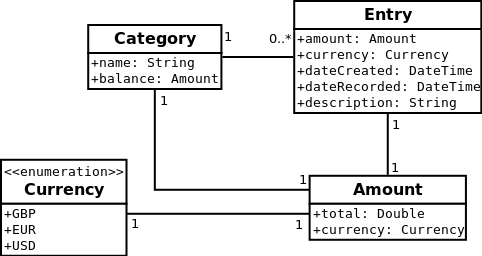
\includegraphics[width=10cm]{./contents/img/Class_Diagram_-_Categories_and_Amount.png}
  \end{center}
  \caption{}
  \label{fig:ClassDiagram.CategoriesAndAmount}
\end{figure}
\FloatBarrier

As implied by the diagram above, the \emph{Category} class will be associated
with instances of the \emph{Entry} class, and will keep track of the balance
made up of the sum of \emph{Amount}'s of each entry. This is done so that the
only way to change the total of a category is by adding positive or negative
entries to it -- for example, to indicate a credit to a category, a negative
entry can be added to it.

Another design choice which can be observed in Figure
\ref{fig:ClassDiagram.CategoriesAndAmount} is that the \emph{Amount} class also
possesses an attribute for currency. This has been designed so as to allow for
the possibility of extending the design to keep track of transactions in
multiple currencies, although it was not a specific requirement. Initially,
there will only be a single default currency which shall be set at runtime.

The next step is to provide a way for these entries to be added to categories.
For this to happen, there needs to be a constraint to ensure that double entry
happens every time a change needs to be made to a category. One of the ways to
achieve this is to apply the \emph{Transaction} pattern
(\cite[][Section~6.2]{fowler1997analysis}):
\begin{figure}[ht!]
  \begin{center}
    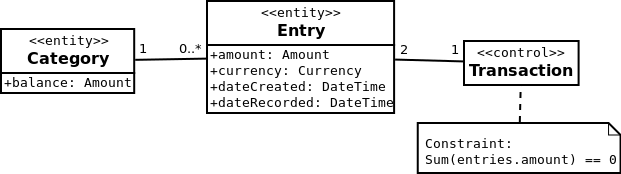
\includegraphics[width=10cm]{./contents/img/Class_Diagram_-_Transaction.png}
  \end{center}
\end{figure}
\FloatBarrier

After having determined the analysis patterns which shall be employed, it makes
sense to dive into a deeper analysis of the use cases described in Chapter
\ref{sec:Requirements}. At this point the objective will be to start modelling
classes based on concepts or things found in the problem domain. This will be
done in the following subsections.


\newpage
\section{Appendix III: How to Build and Run the Application} \label{appendix3}

This is also available from the GitHub Repository for this project,
\href{https://github.com/claudiusbr/personal_finance_system}{here}.

As this is a list of instructions, some of it will be in an imperative voice.

\subsection{What is needed}
\begin{itemize}
  \item
    SBT 1.1.1 (can be downloaded using SDKMAN -- \href{http://sdkman.io/}{http://sdkman.io/})

  \item
    Scala 2.12.4 (can be downloaded with SBT, or using SDKMAN -- 
    \href{http://sdkman.io/}{http://sdkman.io/})

  \item
    MySQL
    \begin{itemize}
      \item
        also, the \texttt{schema.sql} file, which should be included in the
        accompanying USB, but also can be downloaded from
        \href{https://github.com/claudiusbr/personal_finance_system/tree/master/code/original_db_schemas/mysql}{the
        GitHub repo}.

      \item
        and the \texttt{test\_schema.sql}, which should also be included in the
        USB stick, or downloaded from
        \href{https://github.com/claudiusbr/personal_finance_system/tree/master/code/original_db_schemas/mysql}{the
        GitHub repo}.
    \end{itemize}

  \item
    The \texttt{config.properties} file for the main application, which is also
    in the USB, or can be downloaded from
    \href{https://github.com/claudiusbr/personal_finance_system/tree/master/code}{the
    GitHub repo}.
    \begin{itemize}
      \item
        within the file, the \texttt{MySqlUrl} property value needs to be
        replaced by the URL of the database using to run it.
    \end{itemize}


  \item
    The \texttt{testprops} and \texttt{testtextfile} files, which are required
    to run the tests (they should be in the USB, or can be downloaded from
    \href{https://github.com/claudiusbr/personal_finance_system/tree/master/code/src/test}{here}.

  \item
    A \texttt{private.properties} file containing the MySQL username and password for
    the user that can access the two database schemas for this project:
    \texttt{personal\_finance\_schema} and \texttt{test\_personal\_finance}

    \begin{lstlisting}[frame=single]
      MySqlUsername=username
      MySqlPassword=password
    \end{lstlisting}

\end{itemize}

\subsection{Building and Running it}
\subsubsection{set up the project}
\begin{itemize}
  \item
    clone or copy the source files into an empty folder, then \texttt{cd} into
    the root folder for the code (the one containing the \texttt{build.sbt} file);

  \item
    create the \texttt{private.properties} file mentioned above, and save it in
    the root folder;

  \item
    make sure the \texttt{config.properties} is in the root directory

  \item
    make sure the \texttt{testprops} and \texttt{testtextfile} files are in the
    \texttt{src/test} directory;

  \item
    add your username and password to it, if you haven't yet;
\end{itemize}


\subsubsection{Set up MySql}
\begin{itemize}
  \item
    create a database schema called \texttt{personal\_finance\_system};

  \item
    create a database schema called \texttt{test\_personal\_finance};

  \item
    give the user on \texttt{private.properties} access to writing to them;

  \item
    Load the schemas into mysql

    \begin{lstlisting}
    $ mysql -u username -p personal_finance_system < schema.sql
    $ mysql -u username -p test_personal_finance < test_schema.sql
    \end{lstlisting}
\end{itemize}


\subsubsection{Run SBT from the root folder}
\begin{lstlisting}
$ cd personal_finance_system/code
$ sbt run
\end{lstlisting}


\subsection{How to use it}
Make sure your bank statements are in a csv format, and that the column names
match the below exactly (non-case sensitive, though):
\begin{lstlisting}
date,description,amount
... , ... , ...
...
\end{lstlisting}

As this tends to be the trend with bank statements (or at least mine), all
income should be negative, and all expenditure positive, so if you are
uploading either bank or credit card statements, make sure all income and
expenditure is exactly with these signs.


\newpage
\section{Appendix IV: Running Tests} \label{appendix4}

To run the tests with SBT, change location to the root folder of the code and
use the command below:
\begin{lstlisting}
$ sbt test
\end{lstlisting}

At the time of writing, the output of running the tests is shown below:
\begin{lstlisting}
cbrasil@onthego:~/ideaProjects/project/code$ sbt test
[info] Loading settings from idea.sbt ...
[info] Loading global plugins from /home/cbrasil/.sbt/1.0/plugins
[info] Updating ProjectRef(uri(``file:/home/cbrasil/.sbt/1.0/plugins/"),
      ``global-plugins")...
[info] Done updating.
[info] Loading project definition from 
      /home/cbrasil/ideaProjects/project/code/project
[info] Updating ProjectRef(uri
      (``file:/home/cbrasil/ideaProjects/project/code/project/"),
      ``code-build")..
[info] one updating.
[info] Loading settings from build.sbt ...
[info] Set current project to PersonalFinanceSystem 
      (in build file:/home/cbrasil/ideaProjects/project/code/)
[info] Compiling 1 Scala source to 
      /home/cbrasil/ideaProjects/project/code/target/scala-2.12/classes...
[info] Done compiling.
[info] InputValidatorTester:
[info] An InputValidator
[info] - should ensure the csv columns are correct
[info] - should ensure that the correct type argument has been passed
[info] AmountTester:
[info] an Amount instance
[info] - should default to GBP if no currency is provided
[info] RegexDateStringParserTester:
[info] String dates passed to the `dateFromString' method of
      DateFormatter
[info] - should be converted from yyyy(/.-)dd(/.-)dd to DateTime
[info] - should be converted from dd(/.-)mm(/.-)yyyy to DateTime
[info] - should cause it to throw an exception if not in any
        of the formats above
[info] InputTester:
[info] an Input object
[info] - should try to load a file from the filesystem and return a 
        Some if it finds it
[info] - should return a None if it does not find it
[info] DateRegistryTester:
[info] A DateRegistry
[info] - should be able to be instantiated with only one argument
[info] PropertiesLoaderTester:
[info] a PropertiesLoader
[info] - should load properties from a file when requested
[info] InputToEntryParserTester:
[info] an EntryParser
[info] - should parse file contents into Entry instances
[info] - should parse the files even if the columns are not in order
[info] - should parse the files even with columns have different headers
[info] - should parse the contents even if they have interpolated commas
[info] TransactionTester:
[info] - should execute the transaction on a single TransactionUnit
[info] - should execute the transaction on multiple transaction units
[info] StringClassifierTester:
[info] A Classifier
[info] - should assign categories to entries when it can find them
[info] - should return return all entries when it cannot find them
[info] - should match against longest matching prefix
[info]   + Given an entry with a prefix which matches more than 
      one pattern 
[info]   + When it is matched against all categories with which it
      could match 
[info]   + Then it should match against the one with longest 
      matching prefix 
[info] CategoryTester:
[info] A Category
[info] - should have a name
[info] - should have an empty list of Entries
[info] - should be allowed to have no patterns
[info] - should fail if no name is passed
[info] EntryTester:
[info] an Entry
[info] - should have an Amount
[info] - should have a constructor which allows it to be created
      with value, dates and description only
[info] - should have a date the entry was created and a date it
      was recorded
[info] TransactionUnitValidatorTester:
[info] - should execute the transaction on a single TransactionUnit
[info] - should execute the transaction on multiple transaction units
[info] a TransactionCategoriesValidator
[info] - should check that there is at least one category
[info] TransactionEntriesValidatorTester:
[info] - should execute the transaction on a single TransactionUnit
[info] - should execute the transaction on multiple transaction units
[info] a TransactionEntriesValidator
[info] - should return Fail if no list of TransactionUnits is given
[info] - should validate entries to ensure they equal zero
[info] PersistenceBridgeTester:
[info] PersistenceBridge with MySql
[info] - should connect to a database
[info] - should retrieve all categories when requested
[info] - should return a single category when requested
[info] - should return nothing the single category requested does
      not exist
[info] - should return the patterns for a category
[info] - should create a category and return true if it works
[info] - should create a category and return the category details
[info] - should create a pattern and return true if it works
[info] - should create entry descriptions
[info] - should retrieve entry descriptions details
[info] - should add entries to the database when requested
[info] - should fail when the entries do not add up to zero
[info] - should close the connection once it is done
[info] Run completed in 1 second, 760 milliseconds.
[info] Total number of tests run: 46
[info] Suites: completed 14, aborted 0
[info] Tests: succeeded 46, failed 0, canceled 0, ignored 0, pending 0
[info] All tests passed.
[success] Total time: 4 s, completed 06-May-2018 10:20:49
\end{lstlisting}

More information on how to run different types of testing with SBT can be found
on \cite[][Ch.~2]{hinojosa2013testing}.


\end{document}
